\section{Assessing Risk Preferences: A Dual-Criterion Approach}
\subsection{Setup and Definitions}
The results of section \ref{return_section} paint very different pictures of retail investors. 
Using the method set forth by \cite{Welch2022} and \cite{Fedyk2024}, analyzed also in section \ref{fedyk_paper_returns}, yields superior returns and similar drawdowns to the market.
They also conclude that the Robinhood crowd has achieved positive alpha when analyzed under different factor models (table VII, IX, X in \cite{Welch2022} and table 16 in \cite{Fedyk2024}). 
These results appear to be in contrast with the existing literature on retail investing, most notably \cite{BarberOdean2000}.

A more fundamental question, however, is whether those returns are attractive once investors' attitudes toward risk are taken into account.
This section evaluates the Robinhood portfolio against its market benchmarks using two complementary criteria.

First, I adopt the constant-relative-risk-aversion (CRRA) framework, in line with the majority of asset pricing work.
\begin{equation}
    U(W) = 
    \begin{cases}
    \frac{W^{1-\gamma}-1}{1-\gamma}, \gamma\neq 1\\
    \ln(W), \gamma = 1
    \end{cases}
    \label{CRRA}
\end{equation}

By computing the expected utility of both the Robinhood and benchmark portfolios over a grid of possible risk aversion ($\gamma$) values,
I identify the cutoff $\gamma^*$ such that a representative CRRA investor is indifferent between the two.
This delivers a concise, parametric summary of how risk preferences may shape portfolio choice.

However, this method cannot deliver precise estimates given the limited sample size. 
I therefore employ another method to directly estimate the risk aversion $\gamma$, 
following the Generalized Method of Moments (GMM) framework introduced by \cite{hansen1982generalized} to find the risk aversion that satisfies the intertemporal Euler Condition, aspresented also in \cite{Cochrane2005}.

\begin{equation}
    \mathbb{E}\left[ \beta \frac{U^\prime(c_{t+1})}{U^\prime(c_{t})}R_{t+1} \right] = 1\
    \label{euler_def}
\end{equation}  
where $R_{t+1}$ is the realized gross return on the asset at time $t+1$, $\beta$ is discount factor, and $U^\prime(\cdot)$ is the derivative of the utility function..

%Second, I apply first- and second-order stochastic dominance tests (FSD and SSD) to the same return distributions.
%This allows to avoid unnecesary, though conventional, assumptions regarding functional forms or parameterisation.
%Log-Normality might well not be respected for different distributions, stochastic dominance tests take into account the shape of empirical CDFs to answer stronger questions. 

\subsection{Expected Utility and Cutoff}
\subsubsection{Sampling Variability and Finite-Sample Limitations}
Identifying a cutoff level of risk aversion provides a clear criterion for the CRRA utility-maximizing investor: 
it is the minimum $\gamma$ at which an alternative strategy becomes preferred to the Robinhood portfolio.
However, the limited size and noise of the sample imply wide conference intervals for the estimated expected utilities at different $\gamma$ levels.
In practice, this remains a useful conceptual framework to understand how risk preference and beliefs may affect portfolio choice, but in limited samples, its numerical outputs are more illustrative than definitive.
However, this method yields precise results in a very specific case I will describe later. 

Formally, we want to find $\gamma^*$ defined as:
\begin{equation}
    \gamma^* = \min\left\{ \gamma_j : \mathbb{E}[U_p(\gamma_j)] \leq \mathbb{E}[U_m(\gamma_j)] \right\}
    \label{gamma_cutoff}
\end{equation}
where $U_p(\cdot)$ is the utility of the Robinhood portfolio, while $U_m(\cdot)$ is the utility of the market portfolio.

In practice, we apply CRRA utility function (\ref{CRRA}) to each gross return observation and then takes the sample average.
The resulting mean serves as the expected utility implied by the investor's revealed choices over the sample period.
Wealth at time $t$ is equal to gross returns, assuming the initial wealth $W$ to be equal to one without loss of generality.

The main problem related to this approach is inherent to the sample we apply it to, having only 539 observations and inclusion of extreme events such as the COVID crash. 
These factors inflate the sample variability of our mean-utility estimates, so much that regardless of whether we use daily returns, various rolling-window horizons, or subperiods, the resulting confidence intervals remain prohibitively wide.
Figure \ref{fig:cutoff} illustrates this well: 
\begin{figure}[H]
    \centering
    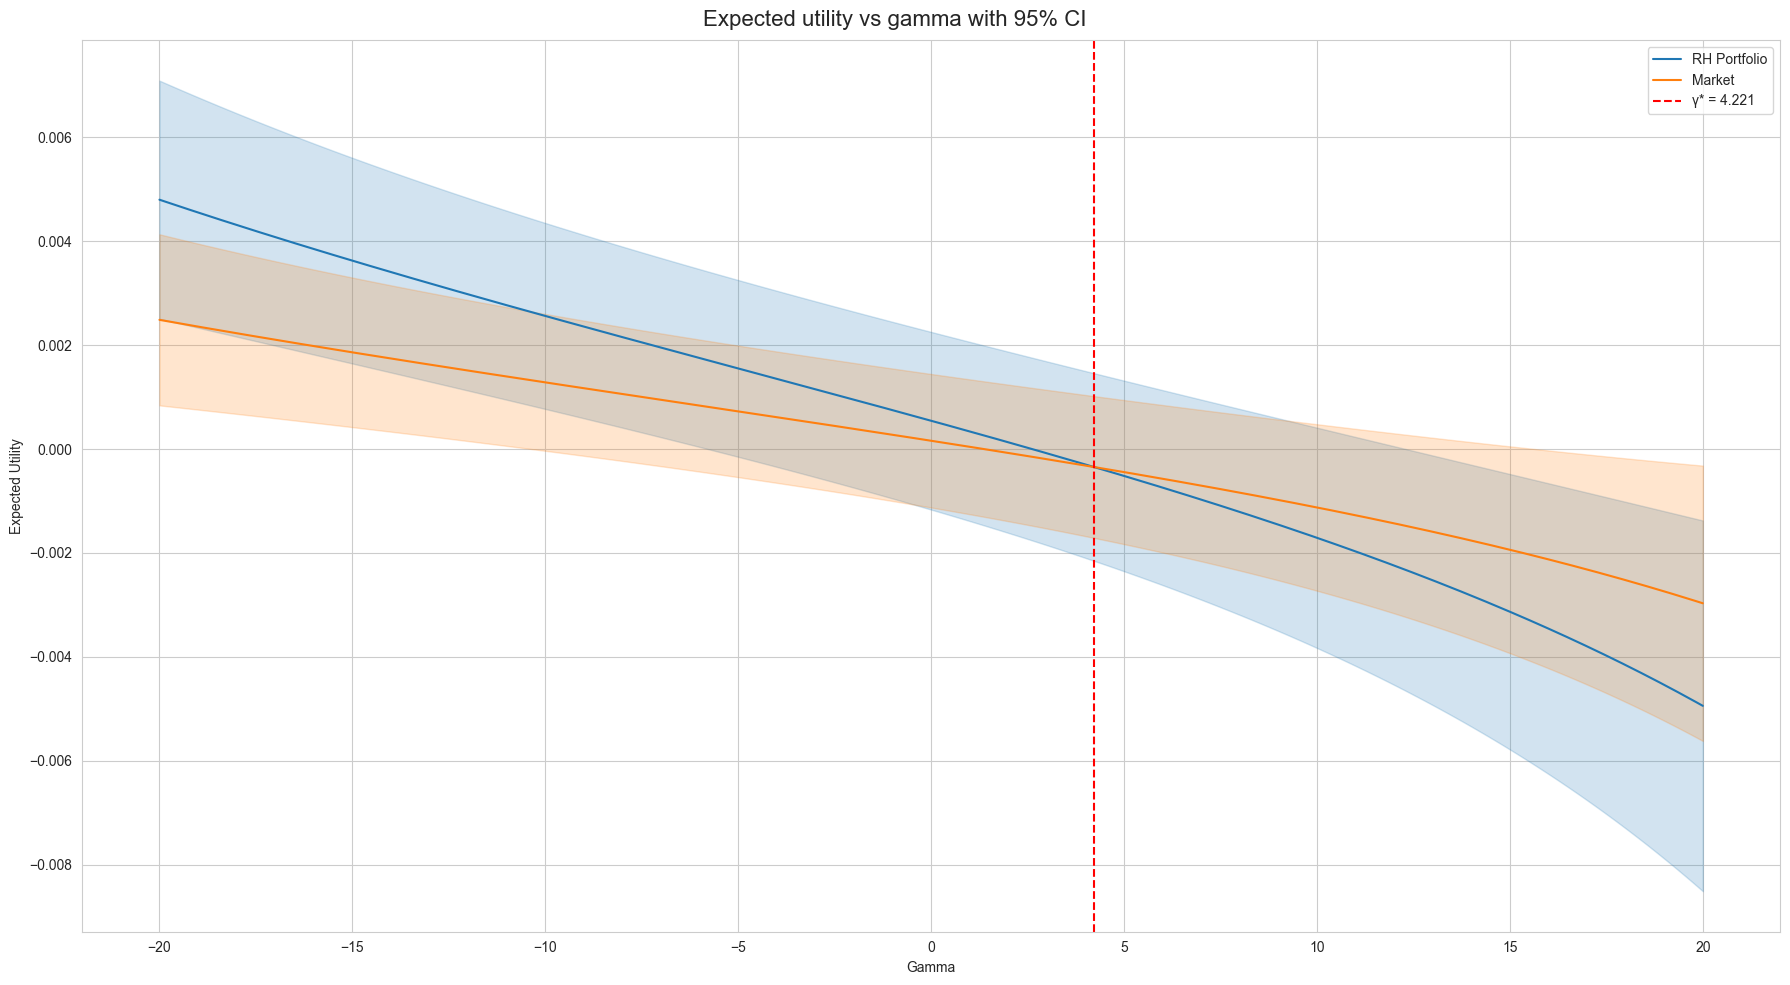
\includegraphics[width=\linewidth]{../images/risk/cutoff_daily.png}
    \caption{Utility for the Robinhood and Market portfolios evaluated over a grid of $\gamma$.}
    \label{fig:cutoff}
\end{figure}

\subsubsection{Augmented Return Sample via All Date-Pairs}
\label{sec:allpairs}
To overcome the limited information in only 539 daily observations, we construct an "all-pairs" dataset that dramatically amplifies our effective sample.  
Specifically, let the trading-day indices in our original series be $1,2,\dots,T$.  
For every ordered pair of dates $(i,j)$ with $1 \le i < j \le T$, we compute the cumulative excess return (net of the risk-free rate) between day $i$ and day $j$ as
\begin{equation}
    R_{i,j}
    \;=\;
    \prod_{k=i+1}^{j}\bigl(1 + r_k - r_{f,k}\bigr),
    \quad
    1 \le i < j \le T,
    \label{eq:allpairs_return}
\end{equation}
where $r_k$ is the portfolio return on day $k$ and $r_{f,k}$ is the daily risk-free rate.  
Using excess returns over the risk-free rate is necessary due to the changes in macroeconomic policy during the time of the sample. 
We treat each multi-day return $R_{i,j}$ as a separate outcome in the investor's distribution of possible holding-period returns, we increase the number of observations from $T$ to $T(T-1)/2$, which reduces sampling variability in our utility-based estimates.  
This "all-pairs" approach preserves the time-ordering of returns while allowing us to evaluate expected utility cutoffs with far greater precision.  

In practice, this results in finding a very low $\gamma^*$ that satisfies equation \ref{gamma_cutoff}, meaning that every investor with a reasonable risk-aversion parameter under CRRA utility would have a greater utility by investing in the market\footnote{
Both the risk-free rate and market returns are downloaded from Kenneth R. French data library \url{https://mba.tuck.dartmouth.edu/pages/faculty/ken.french/data_library.html}}.
In some cases, particularly when ending the sample before the pandemic, the utility curves fitted on the "all-pairs" dataset simply do not intersect for a wide grid of possible risk aversion,
and in fact we find also that in these cases the market stochastically dominates the robinhood portfolio (something which will be analyzed more in depth later).

Performing this exercise for the whole period on the two alternative Robinhood portfolios yields very telling results.
In both instances the cutoff risk aversion as defined in \ref{gamma_cutoff} is negative; 
in particular, the portfolio I constructed has a cutoff risk aversion of -5.437 while the one built using the alternative method we obtain -5.239.
The plot below shows this finding, only extremely risk loving investors would prefer the Robinhood portfolios over a diversified index.  

\begin{figure}[H]
  \centering
  \subfloat[Robinhood Returns Built from Prices]{%
    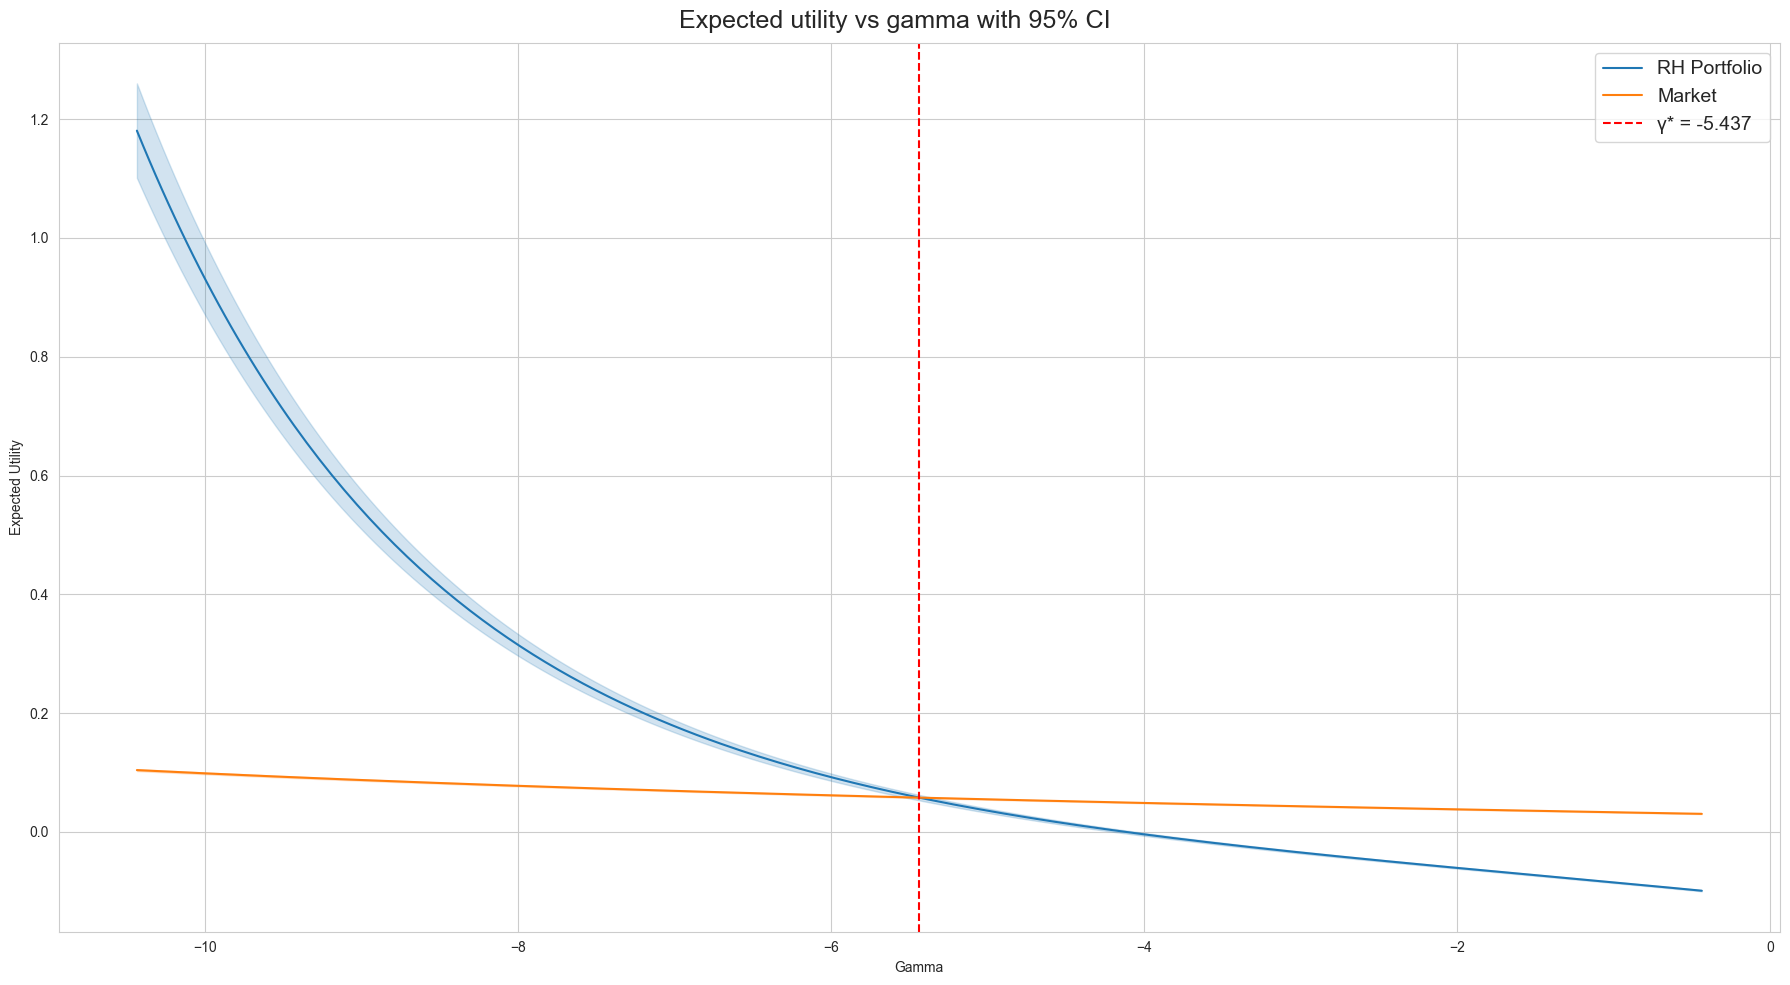
\includegraphics[width=0.48\textwidth]{../images/risk/cutoff_number_all.png}%
    \label{fig:cutoff_number_all}
  }
  \hfill
  \subfloat[Robinhood Returns Built Following Fedyk]{%
    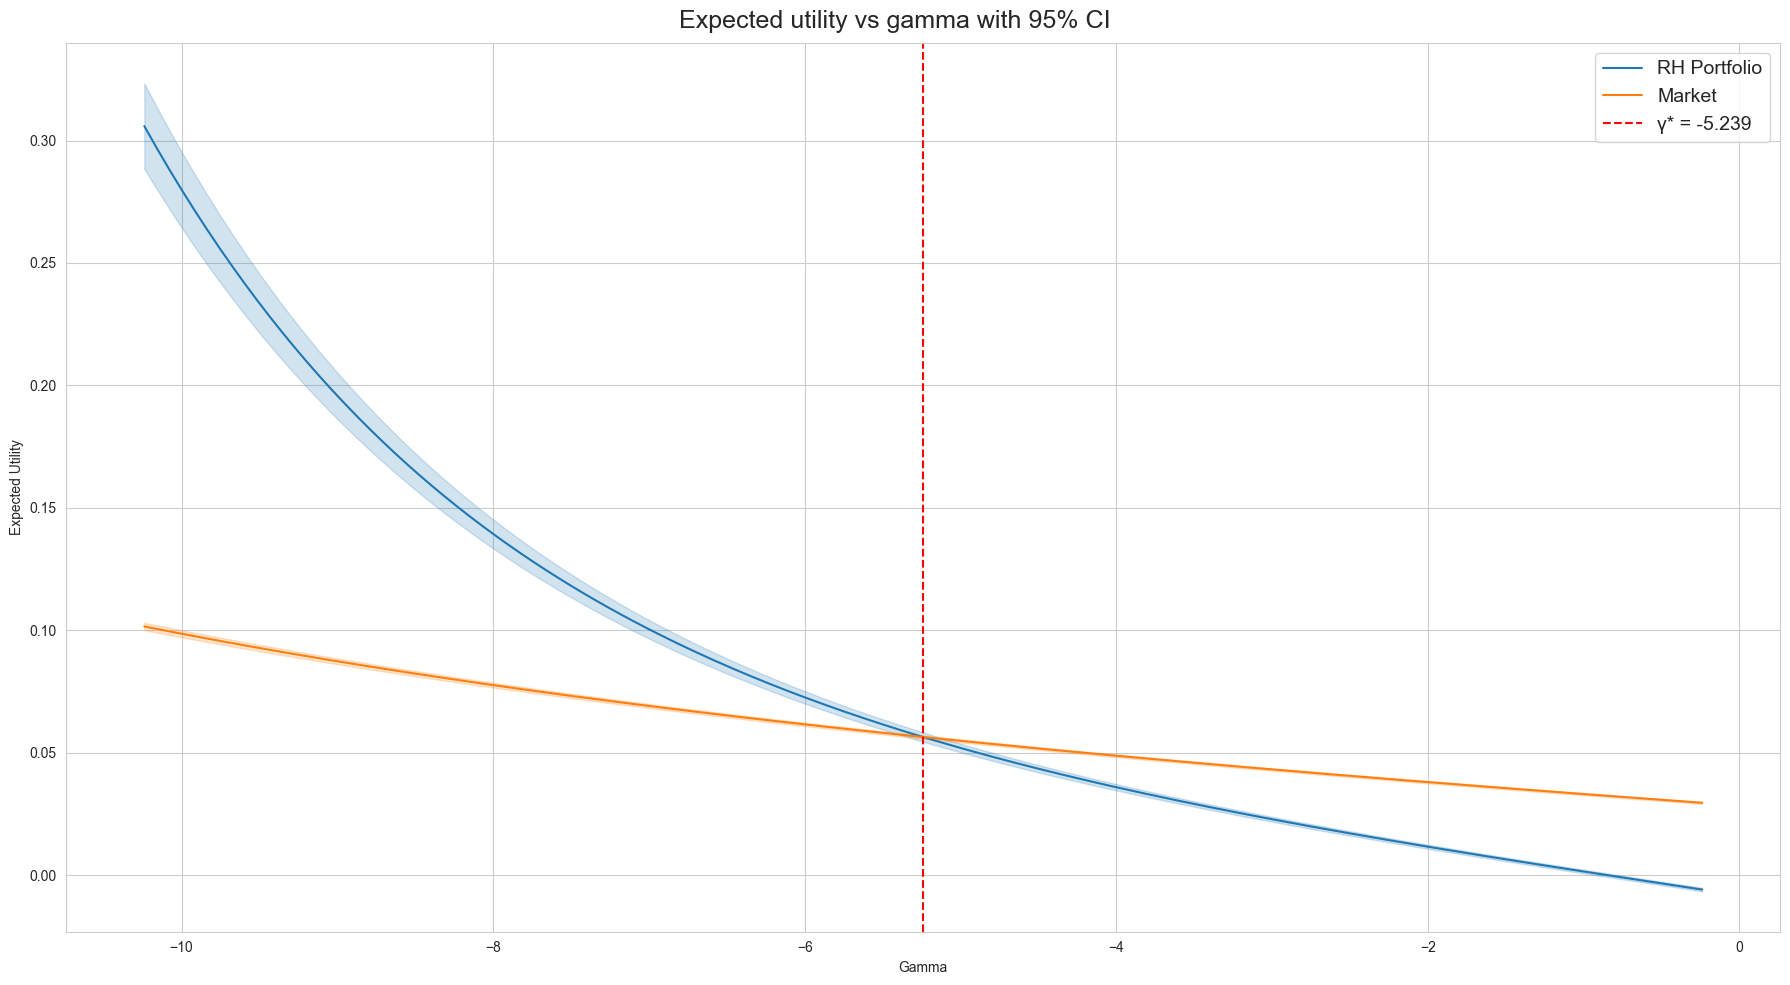
\includegraphics[width=0.48\textwidth]{../images/risk/cutoff_wealth_all.png}%
    \label{fig:cutoff_wealth_all}
  }
  \caption{Expected Utility and Cutoff Risk-aversion for the Robinhood and Market Portfolio.}
  \label{fig:cutoff_all_sidebyside}
\end{figure}

The only case in which $\gamma^*$ is positive is when we compare the Fedyk Portfolio and the World equity ETF as a proxy for the market index, obtaining a value of 1.214.
This implies that weakly risk-averse and risk-loving investors would have a greater utility by investing in this index.
However, if we limit the analysis to the pre-COVID period, the utility of the World ETF strictly dominates for each $\gamma\geq-15.813$, 
highlighting that the former result might indeed be a result of the volatility experienced in early 2020.  

\subsection{Euler Condition Approach to CRRA Parameter Estimation}
\subsubsection{Bootstrap Methodology for GMM-Based $\gamma$ Estimation}
To address the limitations of our cutoff $\gamma$ approach, we turn to the canonical Euler-equation estimator of risk aversion as presented in Chapter 1 of \cite{Cochrane2005}.  
In that framework, the agent's first-order condition for optimal intertemporal consumption and portfolio choice requires \ref{euler_def} to hold.

Rewriting equation \ref{euler_def} and assuming CRRA utility we arrive at the following condition\footnote{Derivation:
$U^\prime(x)=x^{-\gamma}$, hence $\frac{U^\prime(c_{t+1})}{U^\prime(c_{t})}=\left(\frac{c_{t+1}}{c_t}\right)^{-\gamma}$}:
\begin{equation}
    \mathbb{E}\left[ \beta \left( \frac{c_{t+1}}{c_{t}} \right)^{-\gamma} R_{t+1} \right] = 1
\end{equation}  

Then, using gross portfolio returns as a proxy of consumption growth and letting $\beta = \frac{1}{1+\bar{r_f}}$ we derive the following GMM moment condition:
\begin{equation}
    g(\gamma) = \mathbb{E} \left[ \frac{R_{t+1}^{-\gamma}}{1+\bar{r}_f}  R_{t+1} - 1\right] = 0
    \label{gmm_condition}
\end{equation}  

I then use a root-solving algorithm to find the $\hat\gamma$ that satisfies equation \ref{gmm_condition}. 

\paragraph{Bootstrap Confidence Intervals.}
The GMM estimator described above yields a single point estimate $\hat\gamma$, but does not indicate its sampling precision.  
To quantify uncertainty, we apply a nonparametric bootstrap: we repeatedly resample our $T$ return observations (with replacement), re-solve the GMM moment condition in each replicate, and record the resulting $\hat\gamma^{(b)}$ values.  
The empirical distribution of $\{\hat\gamma^{(b)}\}_{b=1}^B$ then provides a straightforward 95\% confidence interval for $\gamma$.  
This approach requires no additional distributional assumptions and directly reflects the finite-sample variability of our risk-aversion estimate.

\subsubsection{Empirical Estimates and Interpretation}
\label{sec:gamma_estimates}
Before describing the results a necessary premise has to be stated.
A key condition for the validity of the nonparametric bootstrap is that the observations be independent and identically distributed (i.i.d.).  
In particular, resampling "with replacement" implicitly treats each data point as a separate draw from the same underlying distribution.  
If the series exhibits serial dependence, as it would be if we used the rolling returns defined in earlier sections, then the standard bootstrap will underestimate sampling variability.  
To avoid this issue we resample the data on weekly and monthly frequencies to estimate risk aversion on different timeframes.

Table \ref{tab:gamma_all} reports our GMM estimates of the CRRA coefficient $\hat\gamma$ alongside 95\% confidence intervals for both the portfolio built on prices (labelled "Mine") and the Fedyk benchmark.  
A few key observations emerge.
At daily and weekly horizons, every point estimate of $\hat\gamma$ is not only strictly positive but also bounded away from zero by its confidence interval.  
This confirms that, under both specifications, the representative investor implied by the Euler-equation GMM is unequivocally risk averse over high-frequency returns.

Moving to monthly returns, the confidence bands widen substantially, now crossing zero, due to the much smaller number of non-overlapping observations.  
While the point estimates remain positive, their CIs reflect that, with only \~18 monthly data points, we lack statistical power to reject mild risk neutrality at conventional levels.

Across all horizons, the "Fedyk" market benchmark yields slightly higher $\hat\gamma$ values than our custom portfolio.  
This suggests that, to satisfy the Euler condition, a representative investor choosing the market must be marginally more risk averse than one choosing the alternative strategy, perhaps compensating for lower volatility or different return skewness.

The strictly positive daily and weekly estimates imply a genuine aversion to risk in the retail investor's revealed preferences.  
In practical terms, these investors require compensation for variance in returns and would, under a fully rational CRRA framework, tilt away from high-variance holdings unless expected excess returns are sufficient.

These findings underscore that the Euler-GMM approach delivers clear, statistically significant evidence of risk aversion at the daily and weekly horizons—where our sample is large enough to pin down a strictly positive $\gamma$.  
It is precisely in these shorter-term windows that we can say with confidence that retail investors reveal genuine aversion to risk.  
As the horizon lengthens and observations dwindle, however, the resulting estimates become too imprecise to draw firm conclusions.


